\documentclass[10pt,aspectratio=169]{beamer}
\usetheme{Madrid}
\usefonttheme{professionalfonts}
\usecolortheme{default}
\usepackage{amsmath,amssymb,bm}
\usepackage{tikz}
\usepackage{booktabs}
\usepackage{listings}
\usepackage{xcolor}
\usepackage{colortbl}
\usetikzlibrary{positioning,arrows.meta,calc,fit}
\definecolor{myblue}{RGB}{31,78,121}
\definecolor{deepblue}{RGB}{20,55,95}
\definecolor{blockblue}{RGB}{42,92,145}
\definecolor{softblue}{RGB}{225,235,245}
\definecolor{mygreen}{RGB}{40,130,90}
\definecolor{myred}{RGB}{180,60,60}
\setbeamercolor{background canvas}{bg=white}
\setbeamercolor{normal text}{fg=black,bg=white}
\setbeamercolor{frametitle}{fg=white,bg=myblue}
\setbeamerfont{frametitle}{series=\bfseries}
\setbeamercolor{title}{fg=white}
\setbeamercolor{subtitle}{fg=white}
\setbeamercolor{author}{fg=black}
\setbeamercolor{date}{fg=black}
\setbeamercolor{structure}{fg=myblue}
\setbeamercolor{item}{fg=myblue}
\setbeamercolor{subitem}{fg=myblue}
\setbeamercolor{enumerate item}{fg=myblue}
\setbeamercolor{block title}{fg=white,bg=myblue}
\setbeamercolor{block body}{fg=black,bg=softblue}
\setbeamercolor{palette primary}{fg=white,bg=myblue}
\setbeamercolor{palette secondary}{fg=white,bg=deepblue}
\setbeamercolor{palette tertiary}{fg=white,bg=deepblue}
\setbeamercolor{palette quaternary}{fg=white,bg=myblue}
\setbeamertemplate{navigation symbols}{}
\setlength{\abovedisplayskip}{4pt}
\setlength{\belowdisplayskip}{4pt}
\setlength{\abovedisplayshortskip}{3pt}
\setlength{\belowdisplayshortskip}{3pt}
\arrayrulecolor{myblue}
\newcommand{\grad}[2]{\frac{\partial #1}{\partial #2}}
\newcommand{\adj}[1]{\bar{#1}}
\tikzset{
    var/.style={
        circle,
        draw=myblue,
        fill=white,
        thick,
        minimum size=0.72cm,
        inner sep=1pt,
        font=\small
    },
    op/.style={
        rectangle,
        draw=mygreen,
        fill=white,
        thick,
        rounded corners,
        minimum width=1.0cm,
        minimum height=0.58cm,
        inner sep=3pt,
        font=\small
    },
    arr/.style={->,thick,myblue,>=Latex},
    barr/.style={->,thick,myred,>=Latex}
}
\lstset{
    basicstyle=\ttfamily\footnotesize,
    breaklines=true,
    columns=fullflexible,
    frame=single,
    rulecolor=\color{myblue},
    backgroundcolor=\color{softblue},
    showstringspaces=false
}
% ---- Python flavouring for the code blocks ----
\lstdefinestyle{py}{
    language=Python,
    keywordstyle=\color{deepblue}\bfseries,
    commentstyle=\color{mygreen}\itshape,
    stringstyle=\color{myred},
    emph={torch,nn,optim,init,F,model,opt,sch},
    emphstyle=\color{blockblue}\bfseries
}
\lstset{style=py}

\AtBeginSection[]{%
  \begin{frame}[plain]
    \vfill
    \centering
    \begin{beamercolorbox}[sep=10pt,center,rounded=true]{block title}
      \usebeamerfont{title}\Large\insertsectionhead
    \end{beamercolorbox}
    \vfill
  \end{frame}
}

\title{Optimizers, Weight Initialization and Weight Decay}
\subtitle{Deep Learning lab}
\author{}
\date{}
\begin{document}

\begin{frame}
\titlepage
\end{frame}

% ------------------------------------------------------------------
\begin{frame}{Overview}
\begin{columns}[c]
\begin{column}{0.54\textwidth}
\begin{enumerate}
    \item[\textcolor{myblue}{\textbf{1.}}] \textbf{Optimizer} \\
          {\small how a gradient becomes a parameter update}
    \vspace{0.25cm}
    \item[\textcolor{myblue}{\textbf{2.}}] \textbf{Initialization} \\
          {\small where the parameters start}
    \vspace{0.25cm}
    \item[\textcolor{myblue}{\textbf{3.}}] \textbf{Weight decay} \\
          {\small how we keep them from growing}
\end{enumerate}
\end{column}
\begin{column}{0.42\textwidth}
\begin{center}
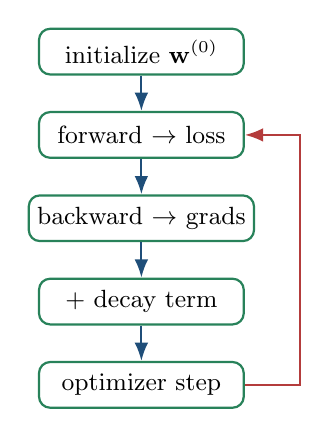
\begin{tikzpicture}[node distance=0.45cm]
\node[op,minimum width=2.6cm] (i) {initialize $\mathbf{w}^{(0)}$};
\node[op,minimum width=2.6cm,below=of i] (f) {forward $\to$ loss};
\node[op,minimum width=2.6cm,below=of f] (b) {backward $\to$ grads};
\node[op,minimum width=2.6cm,below=of b] (d) {+ decay term};
\node[op,minimum width=2.6cm,below=of d] (s) {optimizer step};
\draw[arr] (i) -- (f);
\draw[arr] (f) -- (b);
\draw[arr] (b) -- (d);
\draw[arr] (d) -- (s);
\draw[barr] (s.east) -- ++(0.7,0) |- (f.east);
\end{tikzpicture}
\end{center}
\end{column}
\end{columns}
\end{frame}

% ------------------------------------------------------------------
\begin{frame}[fragile]{Setup}
\begin{lstlisting}
import torch, torch.nn as nn, torch.nn.functional as F
import torch.optim as optim
import torch.nn.init as init

torch.manual_seed(0)
device = "cuda" if torch.cuda.is_available() else "cpu"

class MLP(nn.Module):
    def __init__(self, d_in=784, d_h=256, d_out=10):
        super().__init__()
        self.fc1 = nn.Linear(d_in, d_h)
        self.bn  = nn.BatchNorm1d(d_h)
        self.fc2 = nn.Linear(d_h, d_out)
    def forward(self, x):
        return self.fc2(F.relu(self.bn(self.fc1(x))))

model = MLP().to(device)
crit  = nn.CrossEntropyLoss()
x = torch.randn(64, 784, device=device)          # fake batch
y = torch.randint(0, 10, (64,), device=device)
\end{lstlisting}
\end{frame}

% ==================================================================
\section{Optimizers}

\begin{frame}{The update rules}
The backward pass gives $\mathbf{g}^{(\tau)} = \nabla E(\mathbf{w}^{(\tau)})$. The optimizer turns that into a step.
\vspace{0.2cm}
\begin{columns}[T]
\begin{column}{0.5\textwidth}
\textbf{SGD}
\[ \mathbf{w}^{(\tau+1)} = \mathbf{w}^{(\tau)} - \eta\, \mathbf{g}^{(\tau)} \]
\vspace{0.1cm}
\textbf{Momentum} (PyTorch form)
\begin{align*}
\mathbf{b}^{(\tau)} &= \mu\, \mathbf{b}^{(\tau-1)} + \mathbf{g}^{(\tau)}\\
\mathbf{w}^{(\tau+1)} &= \mathbf{w}^{(\tau)} - \eta\, \mathbf{b}^{(\tau)}
\end{align*}
\end{column}
\begin{column}{0.5\textwidth}
\textbf{Adam} --- a step size per parameter
\begin{align*}
\mathbf{s}^{(\tau)} &= \beta_1 \mathbf{s}^{(\tau-1)} + (1-\beta_1)\mathbf{g}^{(\tau)}\\
\mathbf{r}^{(\tau)} &= \beta_2 \mathbf{r}^{(\tau-1)} + (1-\beta_2)\big(\mathbf{g}^{(\tau)}\big)^2\\
\mathbf{w}^{(\tau+1)} &= \mathbf{w}^{(\tau)} - \eta\,
   \frac{\hat{\mathbf{s}}^{(\tau)}}{\sqrt{\hat{\mathbf{r}}^{(\tau)}}+\varepsilon}
\end{align*}
{\small Hats denote bias correction, $\hat{\mathbf{s}}^{(\tau)} = \mathbf{s}^{(\tau)}/(1-\beta_1^{\tau})$.}
\end{column}
\end{columns}
\vspace{0.25cm}
\begin{block}{The one structural idea}
Everything beyond plain SGD is \emph{extra state per parameter}: a momentum buffer, a
second-moment buffer, or both. That state lives in the optimizer, not in the model.
\end{block}
\end{frame}


\begin{frame}{AdaGrad}
  \vspace{-0.3em}
  \[
    r^{(\tau)}_i = r^{(\tau-1)}_i
      + \left(\frac{\partial E}{\partial w_i}\right)^{2} ,
    \qquad
    \mathbf{w}^{(\tau)}_i = \mathbf{w}^{(\tau-1)}_i
      - \frac{\eta}{\sqrt{r_i} + \varepsilon}
        \left(\frac{\partial E}{\partial w_i}\right)
  \]
  \vspace{-0.6em}
  \begin{itemize}\itemsep0.3em
    \item Each parameter accumulates the sum of its own squared
          gradients, from $r^{(0)}_i = 0$
    \item Parameters that have seen large gradients --- high curvature
          --- have their rates reduced most
    \item \alert{The flaw}: $r_i$ accumulates from the first step and
          never forgets, so the steps eventually become too small and
          learning stalls
  \end{itemize}
  \srcline{Duchi, Hazan \& Singer (2011); Bishop \& Bishop (2024),
  Eqs.~7.39--7.40.}
\end{frame}

\begin{frame}{RMSProp}
  \vspace{-0.3em}
  \[
    r^{(\tau)}_i = \beta\, r^{(\tau-1)}_i
      + (1-\beta)\left(\frac{\partial E}{\partial w_i}\right)^{2} ,
    \qquad
    \mathbf{w}^{(\tau)}_i = \mathbf{w}^{(\tau-1)}_i
      - \frac{\eta}{\sqrt{r_i} + \varepsilon}
        \left(\frac{\partial E}{\partial w_i}\right)
  \]
  \vspace{-0.5em}
  \begin{itemize}\itemsep0.4em
    \item One change from AdaGrad: the running \emph{sum} becomes a
          running \emph{average}, with $0 < \beta < 1$ and typically
          $\beta = 0.9$
    \item The estimate now forgets on a timescale of about
          $1/(1-\beta)$ steps, so it tracks the curvature the iterate is
          currently in
    \item The learning rate can go back up when the surface flattens,
          which is exactly what AdaGrad could not do
  \end{itemize}
  \srcline{Hinton (2012); Bishop \& Bishop (2024), Eqs.~7.41--7.42.}
\end{frame}

\begin{frame}{Adam}
  \vspace{-0.55em}
  \begin{columns}[T, onlytextwidth]
    \begin{column}{0.485\textwidth}
      \[ s^{(\tau)}_i = \beta_1 s^{(\tau-1)}_i
         + (1-\beta_1)\frac{\partial E}{\partial w_i} \]
    \end{column}
    \begin{column}{0.50\textwidth}
      \[ r^{(\tau)}_i = \beta_2 r^{(\tau-1)}_i
         + (1-\beta_2)\left(\frac{\partial E}{\partial w_i}\right)^{2} \]
    \end{column}
  \end{columns}
  \vspace{-0.55em}
  \begin{columns}[T, onlytextwidth]
    \begin{column}{0.30\textwidth}
      \[ \hat s_i = \frac{s^{(\tau)}_i}{1-\beta_1^{\tau}} \]
    \end{column}
    \begin{column}{0.30\textwidth}
      \[ \hat r_i = \frac{r^{(\tau)}_i}{1-\beta_2^{\tau}} \]
    \end{column}
    \begin{column}{0.38\textwidth}
      \[ \mathbf{w}^{(\tau)}_i = \mathbf{w}^{(\tau-1)}_i
         - \frac{\eta\,\hat s_i}{\sqrt{\hat r_i} + \varepsilon} \]
    \end{column}
  \end{columns}
  \vspace{0.1em}
  \begin{itemize}\itemsep0.3em
    \item RMSProp with momentum: an exponential average of the gradient
          \emph{and} of its square. The name is short for
          \alert{adaptive moment estimation}
    \item Typical values are $\beta_1 = 0.9$ and $\beta_2 = 0.99$
    \item The most widely used training algorithm in deep learning
  \end{itemize}
  \srcline{Kingma \& Ba (2015); Bishop \& Bishop (2024),
  Eqs.~7.43--7.47.}
\end{frame}


% ------------------------------------------------------------------
\begin{frame}{Choosing an optimizer}
\begin{center}
\footnotesize
\begin{tabular}{@{}llll@{}}
\toprule
\textbf{Optimizer} & \textbf{Extra state} & \textbf{Typical $\eta$} & \textbf{Use it when}\\
\midrule
\texttt{SGD} & none & $10^{-1}$ & baseline, convex-ish problems\\
\texttt{SGD(momentum=0.9)} & 1 buffer & $10^{-1}$ & CNNs from scratch, best final accuracy\\
\texttt{Adagrad} & sum of $\mathbf{g}^2$ & $10^{-2}$ & sparse features; lr decays forever\\
\texttt{RMSprop} & EMA of $\mathbf{g}^2$ & $10^{-2}$ & RNNs, RL\\
\texttt{Adam} & $\mathbf{s}$ and $\mathbf{r}$ & $10^{-3}$ & fast, forgiving default\\
\texttt{AdamW} & $\mathbf{s}$ and $\mathbf{r}$ & $10^{-3}$--$10^{-4}$ & transformers, anything regularized\\
\texttt{LBFGS} & history & --- & tiny full-batch problems only\\
\bottomrule
\end{tabular}
\end{center}
\vspace{0.35cm}
\begin{itemize}
    \item Adam converges faster early; tuned SGD+momentum often generalizes better on vision.
    \item Adam and AdamW store two extra tensors per parameter, so $3\times$ the model size in memory.
    \item A safe default is AdamW at \texttt{3e-4}.
\end{itemize}
\end{frame}

% ------------------------------------------------------------------
\begin{frame}[fragile]{The training loop}
\begin{lstlisting}
opt = optim.SGD(model.parameters(), lr=0.1, momentum=0.9)

for epoch in range(epochs):
    model.train()
    for xb, yb in loader:
        xb, yb = xb.to(device), yb.to(device)

        opt.zero_grad(set_to_none=True)   # 1. clear old grads
        out  = model(xb)                  # 2. forward
        loss = crit(out, yb)              # 3. loss
        loss.backward()                   # 4. fills p.grad
        opt.step()                        # 5. updates p
\end{lstlisting}
\begin{itemize}
    \item \texttt{backward()} \emph{accumulates} into \texttt{p.grad}; it never clears it. Hence step 1.
    \item \texttt{opt.step()} reads \texttt{p.grad} and mutates \texttt{p} in place, under \texttt{no\_grad}.
\end{itemize}
\end{frame}

% ------------------------------------------------------------------
\begin{frame}[fragile]{The optimizer object}
\begin{lstlisting}
opt = optim.SGD(model.parameters(), lr=0.1, momentum=0.9)

len(opt.param_groups)            # 1
opt.param_groups[0].keys()
# dict_keys(['params', 'lr', 'momentum', 'dampening',
#            'weight_decay', 'nesterov', 'maximize', ...])

opt.param_groups[0]["lr"]        # 0.1
opt.param_groups[0]["lr"] = 0.05 # change lr by hand, any time
\end{lstlisting}
\begin{block}{Mental model}
An optimizer is a list of \emph{param groups}. Each group is a list of tensors plus the
hyperparameters that apply to them. Per-layer learning rates, no-decay lists and freezing are
all just a matter of building the right groups.
\end{block}
\end{frame}

% ------------------------------------------------------------------
\begin{frame}[fragile]{Common mistakes}
\begin{lstlisting}
opt = optim.SGD(model, lr=0.1)         # 1. TypeError:
                                       # pass model.parameters()

for xb, yb in loader:                  # 2. no zero_grad ->
    loss = crit(model(xb), yb)         # grads pile up across
    loss.backward(); opt.step()        # batches, loss explodes

opt.step(); loss.backward()            # 3. step before backward
                                       # -> None grads / no-op

loss.backward(); loss.backward()       # 4. RuntimeError: graph
                                       # freed (use retain_graph)

model.fc2 = nn.Linear(256, 10)         # 5. new tensor, but opt
opt.step()                             # still holds the old one
\end{lstlisting}
\end{frame}

% ------------------------------------------------------------------
\begin{frame}[fragile]{SGD options}
\begin{lstlisting}
# plain SGD
optim.SGD(model.parameters(), lr=0.1)

# heavy-ball momentum:  b <- mu*b + g ;  p <- p - lr*b
optim.SGD(model.parameters(), lr=0.1, momentum=0.9)

# Nesterov: look-ahead gradient (needs momentum>0, dampening=0)
optim.SGD(model.parameters(), lr=0.1, momentum=0.9,
          nesterov=True)

# dampening scales the incoming gradient: b <- mu*b + (1-d)*g
optim.SGD(model.parameters(), lr=0.1, momentum=0.9,
          dampening=0.1)
\end{lstlisting}
PyTorch applies momentum \emph{after} the gradient, so the effective step size is roughly
$\eta/(1-\mu)$. Going from \texttt{momentum=0} to \texttt{0.9} multiplies your effective lr by
about 10 --- reduce \texttt{lr} to match.
\end{frame}

% ------------------------------------------------------------------
\begin{frame}[fragile]{Adaptive optimizers}
\begin{lstlisting}
optim.Adam(model.parameters(), lr=1e-3,
           betas=(0.9, 0.999), eps=1e-8)

optim.AdamW(model.parameters(), lr=1e-3,
            weight_decay=1e-2)        # decoupled decay

optim.RMSprop(model.parameters(), lr=1e-2, alpha=0.99)
optim.Adagrad(model.parameters(), lr=1e-2)


\end{lstlisting}

% # LBFGS re-evaluates the loss, so it needs a closure
% opt =   optim.LBFGS(model.parameters(), lr=0.1)
% def closure():
%     opt.zero_grad()
%     loss = crit(model(x), y)
%     loss.backward()
%     return loss
% opt.step(closure)
On CUDA, \texttt{fused=True} fuses the update into one kernel and is noticeably faster for large
models.
\end{frame}

% ------------------------------------------------------------------
\begin{frame}[fragile]{Optimizer state}
\begin{lstlisting}
opt = optim.Adam(model.parameters(), lr=1e-3)

opt.zero_grad(set_to_none=True)
crit(model(x), y).backward()
opt.step()                      # state is created on first step

p = model.fc1.weight
opt.state[p].keys()
# dict_keys(['step', 'exp_avg', 'exp_avg_sq'])
opt.state[p]["exp_avg"].shape   # torch.Size([256, 784])

sd = opt.state_dict()
sd.keys()                       # dict_keys(['state','param_groups'])
\end{lstlisting}
\begin{itemize}
    \item \texttt{exp\_avg} is $\mathbf{s}$, \texttt{exp\_avg\_sq} is $\mathbf{r}$. That is the whole of Adam.
    \item \texttt{state} stays empty until the first \texttt{step()} --- a useful sanity check.
\end{itemize}
\end{frame}

% ------------------------------------------------------------------
\begin{frame}[fragile]{Per-layer learning rates}
\begin{lstlisting}
opt = optim.SGD([
    {"params": model.fc1.parameters(), "lr": 1e-2},
    {"params": model.bn.parameters(),  "lr": 1e-3},
    {"params": model.fc2.parameters()},        # inherits default
], lr=1e-1, momentum=0.9)

for i, g in enumerate(opt.param_groups):
    print(i, g["lr"], len(g["params"]))
# 0 0.01 2
# 1 0.001 2
# 2 0.1 2

# classic fine-tuning pattern: small lr for the backbone
opt = optim.AdamW([
    {"params": backbone.parameters(), "lr": 1e-5},
    {"params": head.parameters(),     "lr": 1e-3},
], weight_decay=1e-2)
\end{lstlisting}
Every parameter may appear in at most one group; a key omitted in a group falls back to the
constructor default.
\end{frame}

% ------------------------------------------------------------------
\begin{frame}[fragile]{Freezing parameters}
\begin{lstlisting}
# 1. stop gradients from being computed at all
model.fc1.requires_grad_(False)

# 2. and do not hand the frozen tensors to the optimizer
opt = optim.SGD([p for p in model.parameters()
                 if p.requires_grad], lr=1e-2, momentum=0.9)

# unfreeze later -> add a group (or rebuild the optimizer)
model.fc1.requires_grad_(True)
opt.add_param_group({"params": model.fc1.parameters(),
                     "lr": 1e-3})
\end{lstlisting}
\begin{block}{Why both steps}
\texttt{requires\_grad=False} alone is usually enough, but with weight decay or momentum a frozen
tensor still inside the optimizer can keep drifting.
\end{block}
\end{frame}

% ------------------------------------------------------------------
\begin{frame}[fragile]{Learning-rate schedulers}
\begin{lstlisting}
from torch.optim.lr_scheduler import (StepLR, MultiStepLR,
    ExponentialLR, CosineAnnealingLR, OneCycleLR,
    ReduceLROnPlateau, LinearLR, SequentialLR)

sch = StepLR(opt, step_size=30, gamma=0.1)      # x0.1 every 30
sch = MultiStepLR(opt, milestones=[60,120], gamma=0.2)
sch = CosineAnnealingLR(opt, T_max=epochs, eta_min=0.0)
sch = OneCycleLR(opt, max_lr=0.1, epochs=epochs,
                 steps_per_epoch=len(loader))
sch = ReduceLROnPlateau(opt, mode="min", factor=0.5,
                        patience=5)

# linear warmup, then cosine
warm = LinearLR(opt, start_factor=0.1, total_iters=5)
cos  = CosineAnnealingLR(opt, T_max=epochs - 5)
sch  = SequentialLR(opt, [warm, cos], milestones=[5])
\end{lstlisting}
A scheduler holds a reference to \texttt{opt} and simply rewrites
\texttt{param\_groups[i]["lr"]}.
\end{frame}

% ------------------------------------------------------------------
\begin{frame}[fragile]{Calling \texttt{scheduler.step()}}
\begin{lstlisting}
# A. per-epoch schedulers: StepLR, CosineAnnealingLR, ...
for epoch in range(epochs):
    train_one_epoch(model, loader, opt, crit)
    sch.step()
    print(epoch, sch.get_last_lr())     # one lr per param group

# B. per-batch schedulers: OneCycleLR, CosineAnnealingWarmRestarts
for xb, yb in loader:
    opt.zero_grad(set_to_none=True)
    crit(model(xb), yb).backward()
    opt.step()
    sch.step()                          # inside the batch loop

# C. metric-driven: ReduceLROnPlateau needs the number
plateau.step(evaluate(model, val_loader, crit))
\end{lstlisting}
\begin{itemize}
    \item Always \texttt{opt.step()} before \texttt{sch.step()}; the reverse order warns and skips an lr.
    \item Calling a per-epoch scheduler once per batch is the most common LR bug.
\end{itemize}
\end{frame}

% ------------------------------------------------------------------
\begin{frame}[fragile]{Gradient clipping and accumulation}
\begin{lstlisting}
# gradient clipping: after backward(), before step()
loss.backward()
gn = torch.nn.utils.clip_grad_norm_(model.parameters(),
                                    max_norm=1.0)
print(gn)                 # the pre-clip total norm -- log this
opt.step()

# gradient accumulation: effective batch = batch_size * K
K = 4
opt.zero_grad(set_to_none=True)
for i, (xb, yb) in enumerate(loader):
    loss = crit(model(xb), yb) / K       # scale the loss
    loss.backward()                      # accumulate
    if (i + 1) % K == 0:
        opt.step()
        opt.zero_grad(set_to_none=True)
\end{lstlisting}
\texttt{clip\_grad\_norm\_} rescales the whole gradient.
% and is what you almost always want;
\texttt{clip\_grad\_value\_} clips element-wise.
\end{frame}

% ------------------------------------------------------------------
\begin{frame}[fragile]{Saving and resuming}
\begin{lstlisting}
torch.save({"epoch": epoch,
            "model": model.state_dict(),
            "opt":   opt.state_dict(),
            "sch":   sch.state_dict()}, "ckpt.pt")

# resume: build model, optimizer and scheduler first
model = MLP().to(device)
opt   = optim.AdamW(model.parameters(), lr=1e-3)
sch   = CosineAnnealingLR(opt, T_max=epochs)

ck = torch.load("ckpt.pt", map_location=device)
model.load_state_dict(ck["model"])
opt.load_state_dict(ck["opt"])     # restores m, v, momentum
sch.load_state_dict(ck["sch"])
\end{lstlisting}
\begin{block}{Why it matters}
Reloading only the model throws away the momentum and second-moment buffers. Training
restarts with a cold optimizer and the loss visibly jumps.
\end{block}
\end{frame}

% ------------------------------------------------------------------
\begin{frame}[fragile]{Comparing optimizers}
\begin{lstlisting}[basicstyle=\ttfamily\scriptsize]
def run(make_opt, steps=300):
    torch.manual_seed(0)                 # same init every run
    m = MLP().to(device)
    o = make_opt(m.parameters())
    hist = []
    for _ in range(steps):
        o.zero_grad(set_to_none=True)
        l = crit(m(x), y)
        l.backward()
        o.step()
        hist.append(l.item())
    return hist

runs = {
  "SGD":     lambda p: optim.SGD(p, lr=0.1),
  "SGD+mom": lambda p: optim.SGD(p, lr=0.1, momentum=0.9),
  "Adam":    lambda p: optim.Adam(p, lr=1e-3),
  "AdamW":   lambda p: optim.AdamW(p, lr=1e-3, weight_decay=1e-2),
}
for name, f in runs.items():
    h = run(f)
    print(f"{name:8s} start={h[0]:.3f}  end={h[-1]:.4f}")
\end{lstlisting}
\end{frame}

% ==================================================================
\section{Weight Initialization}

\begin{frame}{Why initialization matters}
For a linear layer with $n_{\text{in}}$ inputs and i.i.d.\ zero-mean weights,
\[
\operatorname{Var}(a_{\ell}) \;\approx\; n_{\text{in}} \operatorname{Var}(w_\ell)\,
\operatorname{Var}(a_{\ell-1}),
\]
so across $L$ layers the activation scale is multiplied by
$\big(n_{\text{in}}\operatorname{Var}(w)\big)^{L}$.
\vspace{0.25cm}
\begin{columns}[T]
\begin{column}{0.5\textwidth}
\begin{block}{Xavier / Glorot --- tanh, sigmoid}
\[ \operatorname{Var}(w)=\frac{2}{n_{\text{in}}+n_{\text{out}}} \]
Balances forward and backward variance.
\end{block}
\end{column}
\begin{column}{0.5\textwidth}
\begin{block}{Kaiming / He --- ReLU}
\[ \operatorname{Var}(w)=\frac{2}{n_{\text{in}}} \]
The extra 2 offsets ReLU zeroing half the activations.
\end{block}
\end{column}
\end{columns}
\vspace{0.25cm}
\begin{itemize}
    \item $n\operatorname{Var}(w)<1$: activations and gradients \textbf{vanish} with depth.
    \item $n\operatorname{Var}(w)>1$: they \textbf{explode}, and the loss becomes \texttt{nan}.
    \item All-zero weights: every neuron in a layer gets an identical gradient forever, so
          \textbf{symmetry is never broken}. Zero \emph{biases} are fine.
\end{itemize}
\end{frame}

% ------------------------------------------------------------------
\begin{frame}[fragile]{PyTorch defaults}
\begin{lstlisting}
lin = nn.Linear(784, 256)
# weight: kaiming_uniform_(w, a=sqrt(5))  ->  U(-k, k)
# bias:   U(-k, k)          with  k = 1 / sqrt(fan_in)
1 / 784**0.5                          # 0.0357
lin.weight.std().item()               # ~0.0206 = k/sqrt(3)

conv = nn.Conv2d(3, 16, 3)            # fan_in = 3*3*3 = 27
conv.weight.std().item()              # ~0.111

nn.BatchNorm1d(256).weight            # all ones  (gamma)
nn.BatchNorm1d(256).bias              # all zeros (beta)
nn.Embedding(1000, 64).weight.std()   # ~1.0  -> N(0, 1)
\end{lstlisting}
The defaults are reasonable but not optimal: the effective gain is $\sqrt{1/3}$, which is
conservative for ReLU networks. Deep ReLU stacks, GANs and transformers all set init
explicitly.
\end{frame}

% ------------------------------------------------------------------
\begin{frame}[fragile]{The \texttt{torch.nn.init} functions}
\begin{lstlisting}
w = torch.empty(256, 784)

init.zeros_(w);  init.ones_(w);  init.constant_(w, 0.01)
init.normal_(w, mean=0.0, std=0.02)
init.uniform_(w, a=-0.1, b=0.1)
init.trunc_normal_(w, std=0.02, a=-0.04, b=0.04)

init.xavier_uniform_(w, gain=1.0)
init.xavier_normal_(w, gain=1.0)
init.kaiming_uniform_(w, mode="fan_in",  nonlinearity="relu")
init.kaiming_normal_(w,  mode="fan_out", nonlinearity="relu")

init.orthogonal_(w, gain=1.0)         # RNNs, very deep nets
init.eye_(torch.empty(64, 64))
\end{lstlisting}
\begin{itemize}
    \item Every function ends in \texttt{\_}: in place, and not tracked by autograd.
    \item \texttt{mode="fan\_in"} preserves the forward variance, \texttt{"fan\_out"} the backward one.
          Vision code usually uses \texttt{fan\_out} for convolutions.
\end{itemize}
\end{frame}

% ------------------------------------------------------------------
\begin{frame}[fragile]{Gain}
\begin{lstlisting}
init.calculate_gain("linear")            # 1.0
init.calculate_gain("sigmoid")           # 1.0
init.calculate_gain("tanh")              # 1.6667  = 5/3
init.calculate_gain("relu")              # 1.4142  = sqrt(2)
init.calculate_gain("leaky_relu", 0.2)   # 1.3868

# kaiming-normal std should equal gain / sqrt(fan_mode)
w = torch.empty(1000, 500)
init.kaiming_normal_(w, nonlinearity="relu")
w.std().item(), (2 / 500)**0.5           # 0.0632, 0.0632

# xavier with an explicit gain
fc = nn.Linear(256, 256)
init.xavier_uniform_(fc.weight,
                     gain=init.calculate_gain("tanh"))
\end{lstlisting}
Checking \texttt{w.std()} against the formula is the quickest way to confirm you initialized what
you meant to.
\end{frame}

% ------------------------------------------------------------------
\begin{frame}[fragile]{Initializing a whole model}
\begin{lstlisting}
def init_weights(m):
    if isinstance(m, nn.Linear):
        init.kaiming_normal_(m.weight, nonlinearity="relu")
        if m.bias is not None:
            init.zeros_(m.bias)
    elif isinstance(m, nn.Conv2d):
        init.kaiming_normal_(m.weight, mode="fan_out",
                             nonlinearity="relu")
    elif isinstance(m, (nn.BatchNorm1d, nn.BatchNorm2d,
                        nn.LayerNorm)):
        init.ones_(m.weight)
        init.zeros_(m.bias)

model.apply(init_weights)      # depth-first over all submodules
\end{lstlisting}
\begin{itemize}
    \item \texttt{apply} calls the function on every submodule and on the model itself, then returns
          the model, so \texttt{model = MLP().apply(init\_weights)} works.
    \item Anything the \texttt{isinstance} chain does not match keeps its default init.
\end{itemize}
\end{frame}

% ------------------------------------------------------------------
\begin{frame}[fragile]{Initializing custom modules}
\begin{lstlisting}
class Block(nn.Module):
    def __init__(self, d):
        super().__init__()
        self.fc = nn.Linear(d, d)
        self.reset_parameters()          # convention: call here
    def reset_parameters(self):
        init.xavier_uniform_(self.fc.weight,
                             gain=init.calculate_gain("tanh"))
        init.zeros_(self.fc.bias)
    def forward(self, z):
        return torch.tanh(self.fc(z))

# name-based sweep, when isinstance is not expressive enough
for name, p in model.named_parameters():
    if p.dim() >= 2:                     # weight matrices
        init.xavier_uniform_(p)
    elif "bias" in name:                 # 1-D: bias, gamma, beta
        with torch.no_grad():
            p.zero_()
\end{lstlisting}
\end{frame}

% ------------------------------------------------------------------
% \begin{frame}[fragile]{Checking activation statistics}
% \begin{lstlisting}[basicstyle=\ttfamily\scriptsize]
% def layer_stats(model, x):
%     acts, hooks = {}, []
%     for name, m in model.named_modules():
%         if isinstance(m, nn.Linear):
%             hooks.append(m.register_forward_hook(
%                 lambda mod, inp, out, n=name:
%                     acts.__setitem__(n, out.detach())))
%     model.eval()
%     with torch.no_grad():
%         model(x)
%     for h in hooks:
%         h.remove()
%     for n, a in acts.items():
%         print(f"{n:6s} mean={a.mean():+.4f} std={a.std():.4f}")

% layer_stats(model, x)
% # healthy : std stays O(1) as depth grows
% # std->0  : vanishing -- gain too small
% # std huge: exploding -- gain too large, expect nan soon
% \end{lstlisting}
% On a 10-layer ReLU MLP, \texttt{normal\_(std=0.01)} drives the activation std toward zero within a
% few layers, while \texttt{kaiming\_normal\_} holds it roughly constant.
% \end{frame}

% ------------------------------------------------------------------
% \begin{frame}[fragile]{Do's and don'ts}
% \begin{columns}[T]
% \begin{column}{0.49\textwidth}
% \textbf{Do}
% \begin{itemize}\small
%     \item Use the in-place \texttt{\_} functions on \texttt{m.weight}.
%     \item Zero the biases; set BN/LN $\gamma=1$, $\beta=0$.
%     \item Match \texttt{nonlinearity} and \texttt{gain} to the activation you actually use.
%     \item Print one \texttt{.std()} to confirm.
% \end{itemize}
% \end{column}
% \begin{column}{0.49\textwidth}
% \textbf{Do not}
% \begin{itemize}\small
%     \item Write \texttt{p = p * 2} --- it rebinds a local name, the model is untouched.
%     \item Reach for \texttt{.data}; use \texttt{torch.no\_grad()}.
%     \item Zero-initialize weight matrices.
%     \item Re-initialize after loading a checkpoint.
% \end{itemize}
% \end{column}
% \end{columns}
% \vspace{0.3cm}
% \begin{lstlisting}[basicstyle=\ttfamily\scriptsize]
% p = model.fc1.weight
% p = p * 2                          # WRONG: no effect on model
% with torch.no_grad(): p.mul_(2)    # right
% init.normal_(p, std=0.02)          # right, and clearer
% \end{lstlisting}
% \end{frame}

% ==================================================================
\section{Weight Decay}

\begin{frame}{$L_2$ regularization and weight decay}
Add an $L_2$ penalty to the objective:
\[
\tilde{E}(\mathbf{w}) = E(\mathbf{w}) + \tfrac{\lambda}{2}\lVert\mathbf{w}\rVert^2
\qquad\Longrightarrow\qquad
\tilde{\mathbf{g}} = \mathbf{g} + \lambda\mathbf{w}.
\]
\vspace{0.1cm}
\begin{columns}[T]
\begin{column}{0.5\textwidth}
\textbf{With SGD} the two views coincide:
\[
\mathbf{w}^{(\tau+1)} = (1-\eta\lambda)\,\mathbf{w}^{(\tau)} - \eta\, \mathbf{g}^{(\tau)}
\]
a plain multiplicative shrink each step.
\end{column}
\begin{column}{0.5\textwidth}
\textbf{With Adam} they do not. Adding $\lambda\mathbf{w}$ to $\mathbf{g}$ means the penalty is then
\emph{divided} by $\sqrt{\hat{\mathbf{r}}}$, so parameters with large gradients get decayed less.
\end{column}
\end{columns}
\vspace{0.25cm}
\begin{block}{AdamW: decoupled weight decay}
\[
\mathbf{w}^{(\tau+1)} = \mathbf{w}^{(\tau)} - \eta\lambda\mathbf{w}^{(\tau)}
- \eta\,\frac{\hat{\mathbf{s}}^{(\tau)}}{\sqrt{\hat{\mathbf{r}}^{(\tau)}}+\varepsilon}
\]
The decay term bypasses the adaptive scaling entirely. This is why $\lambda$ for AdamW
($0.01$--$0.1$) looks nothing like $\lambda$ for SGD ($10^{-4}$--$10^{-3}$).
\end{block}
\end{frame}

% ------------------------------------------------------------------
\begin{frame}[fragile]{The \texttt{weight\_decay} argument}
\begin{lstlisting}
# SGD: g <- g + wd * p   (== true L2, thanks to no adaptivity)
optim.SGD(model.parameters(), lr=0.1, momentum=0.9,
          weight_decay=5e-4)

# Adam: coupled L2 -- legal, but rarely what you want
optim.Adam(model.parameters(), lr=1e-3, weight_decay=1e-2)

# AdamW: decoupled -- p <- p - lr * wd * p
optim.AdamW(model.parameters(), lr=1e-3, weight_decay=1e-2)

# turn decay off mid-training
for g in opt.param_groups:
    g["weight_decay"] = 0.0
\end{lstlisting}
The default is \texttt{weight\_decay=0.0} for every optimizer. If you never pass it, you get no
regularization from this route at all.
\end{frame}

% ------------------------------------------------------------------
\begin{frame}[fragile]{Built-in vs.\ manual penalty}
\begin{lstlisting}
wd = 5e-4

# A. built-in: no penalty term in the graph, cheapest
opt = optim.SGD(model.parameters(), lr=0.1, weight_decay=wd)
loss = crit(model(x), y)
loss.backward(); opt.step()

# B. by hand: the loss you print now includes the penalty
opt = optim.SGD(model.parameters(), lr=0.1)
l2  = sum(p.pow(2).sum() for p in model.parameters())
loss = crit(model(x), y) + 0.5 * wd * l2
loss.backward(); opt.step()

# C. L1 has no optimizer flag -- by hand is the only way
l1 = sum(p.abs().sum() for p in model.parameters())
loss = crit(model(x), y) + 1e-5 * l1
\end{lstlisting}
A and B give identical updates for SGD, and A is faster. Never do both --- that applies decay
twice.
\end{frame}

% ------------------------------------------------------------------
\begin{frame}[fragile]{Excluding biases and norm layers}
\begin{lstlisting}
def param_groups(model, wd=1e-2):
    decay, no_decay = [], []
    for name, p in model.named_parameters():
        if not p.requires_grad:
            continue
        if p.ndim <= 1 or name.endswith(".bias"):
            no_decay.append(p)     # biases, BN/LN gamma & beta
        else:
            decay.append(p)        # weight matrices, conv kernels
    return [{"params": decay,    "weight_decay": wd},
            {"params": no_decay, "weight_decay": 0.0}]

opt = optim.AdamW(param_groups(model, wd=1e-2), lr=3e-4)
\end{lstlisting}
\begin{itemize}
    \item Shrinking a BatchNorm $\gamma$ toward 0 kills the layer's output scale; shrinking a bias
          just removes a free offset. Neither helps generalization.
    \item The \texttt{p.ndim <= 1} test catches biases and all norm parameters in one line.
\end{itemize}
\end{frame}

% ------------------------------------------------------------------
\begin{frame}[fragile]{Effect on the weight norm}
\begin{lstlisting}[basicstyle=\ttfamily\scriptsize]
def wnorm(m):
    return torch.sqrt(sum(p.pow(2).sum()
                          for p in m.parameters()
                          if p.ndim >= 2)).item()

for tag, wd in [("wd=0", 0.0), ("wd=1e-2", 1e-2),
                ("wd=1e-1", 1e-1)]:
    torch.manual_seed(0)
    m = MLP().to(device)
    o = optim.AdamW(m.parameters(), lr=1e-3, weight_decay=wd)
    for _ in range(400):
        o.zero_grad(set_to_none=True)
        loss = crit(m(x), y)
        loss.backward()
        o.step()
    print(f"{tag:8s} loss={loss.item():.4f} ||W||={wnorm(m):.2f}")
\end{lstlisting}
Larger \texttt{wd} raises the training loss while shrinking $\lVert\mathbf{w}\rVert$. That trade is the
whole point, so judge it on validation accuracy, never on training loss.
\end{frame}

% % ------------------------------------------------------------------
% \begin{frame}{Typical values}
% \begin{center}
% \footnotesize
% \begin{tabular}{@{}llll@{}}
% \toprule
% \textbf{Setting} & \textbf{Optimizer} & \textbf{lr $\eta$} & \textbf{weight decay $\lambda$}\\
% \midrule
% Small MLP, tabular data      & Adam    & $10^{-3}$              & $0$ or $10^{-4}$\\
% CNN from scratch (bs 256)    & SGD, mom.\ $0.9$ & $0.1$ + cosine & $5\times10^{-4}$\\
% Fine-tune a CNN backbone     & SGD, mom.\ $0.9$ & $10^{-2}$      & $10^{-4}$\\
% Transformer from scratch     & AdamW   & $1$--$3\times10^{-4}$, warmup & $0.1$\\
% Fine-tune a pretrained LM    & AdamW   & $2$--$5\times10^{-5}$  & $0.01$\\
% GAN generator / discriminator& Adam, $\beta_1{=}0.5$ & $2\times10^{-4}$ & $0$\\
% \bottomrule
% \end{tabular}
% \end{center}
% \vspace{0.4cm}
% \begin{itemize}
%     \item Tune \textbf{lr first}, on a log grid. It matters far more than anything else here.
%     \item lr and weight decay interact: in SGD the shrink per step is $\eta\lambda$, so halving
%           the lr halves the effective regularization.
%     \item Excluding biases and norm parameters is worth a few tenths of a percent for free.
% \end{itemize}
% \end{frame}

% ==================================================================
\section{Putting it together}

\begin{frame}[fragile]{Complete example (1/2)}
\begin{lstlisting}[basicstyle=\ttfamily\scriptsize]
model = MLP().to(device)

# --- 1. initialization -------------------------------------------
def init_weights(m):
    if isinstance(m, nn.Linear):
        init.kaiming_normal_(m.weight, nonlinearity="relu")
        init.zeros_(m.bias)
    elif isinstance(m, nn.BatchNorm1d):
        init.ones_(m.weight); init.zeros_(m.bias)
model.apply(init_weights)

# --- 2. weight decay: everything except biases and BN ------------
decay    = [p for p in model.parameters() if p.ndim >= 2]
no_decay = [p for p in model.parameters() if p.ndim < 2]
groups = [{"params": decay,    "weight_decay": 1e-2},
          {"params": no_decay, "weight_decay": 0.0}]

# --- 3. optimizer and schedule -----------------------------------
opt = optim.AdamW(groups, lr=3e-4)
sch = torch.optim.lr_scheduler.CosineAnnealingLR(opt, T_max=EPOCHS)
\end{lstlisting}
% Three blocks of setup for the three topics. None of it touches the training loop.
\end{frame}

% ------------------------------------------------------------------
\begin{frame}[fragile]{Complete example (2/2)}
\begin{lstlisting}[basicstyle=\ttfamily\scriptsize]
for epoch in range(EPOCHS):
    model.train()
    for xb, yb in loader:
        xb, yb = xb.to(device), yb.to(device)
        opt.zero_grad(set_to_none=True)
        loss = crit(model(xb), yb)
        loss.backward()
        torch.nn.utils.clip_grad_norm_(model.parameters(), 1.0)
        opt.step()
    sch.step()

    model.eval()
    with torch.no_grad():
        acc = sum((model(xb.to(device)).argmax(1) == yb.to(device))
                  .sum().item() for xb, yb in val_loader) / n_val
    print(f"ep {epoch}  loss {loss.item():.4f} "
          f"acc {acc:.3f}  lr {sch.get_last_lr()[0]:.2e}")
\end{lstlisting}
\begin{itemize}
    \item \texttt{model.train()} and \texttt{model.eval()} matter here because of BatchNorm.
    % \item Log the lr every epoch. If a schedule is silently doing nothing, this is how you find out.
\end{itemize}
\end{frame}

\end{document}